\documentclass{article}
\title{Matrix Equation Solvers}
\author{Alex Harvey - mm13ah - ID: 200786528}
\date{}

\usepackage{amsmath}
\numberwithin{equation}{section}
\usepackage{amssymb}
\usepackage{amsthm}
\usepackage{blindtext}
\usepackage[parfill]{parskip}
\usepackage{graphicx}
\usepackage{textcomp}
\usepackage[utf8]{inputenc}
\usepackage{float}
\usepackage{diagbox}
\usepackage{tikz}
\usepackage{pgfgantt}
\usepackage{nicefrac}
\usepackage{caption}

\begin{document}

\maketitle

\newpage

\tableofcontents

\clearpage

\section{Introduction}
\subsection{Problem Statement}

The traditional approach to solving partial differential equations numerically involves stacking all the unknowns of the problem into a single vector which ignores underlying structures. This prevents methods from being used which can take advantage of the problem structure to solve the problem more efficiently. This can come at a significant cost when uncertainty is introduced into the system. An alternative approach is to formulate the problem as a matrix equation, which can be solved using a range of different methods. This project involves exploring how this alternative formulation can be solved using matrix solvers, and how these solvers compare against each other. 

As an example, define spatial domain $\mathcal{D} = \{(x,y) : 0 \leq x \leq 1, \; 0 \leq y \leq 1 \}$ and let $u: \mathcal{D} \to \mathbb{R}$ be the solution of the equation:
	\begin{equation} 
	-u_{xx} - u_{yy} = f
	\end{equation}
with boundary conditions $u(x,y)=0$, as shown in Figure 1.

\begin{figure}[H]
\begin{tikzpicture}
\draw (0,0) rectangle (6,6);
\node at (3,3) {$-u_{xx}-u_{yy}=f$};
\node at (-0.25,3) {$0$};
\node at (6.25,3) {$0$};
\node at (3,-0.25) {$0$};
\node at (3,6.25) {$0$};

\node at (-0.25,-0.25) {$(0,0)$};
\node at (-0.25,6.25) {$(0,1)$};
\node at (6.25,-0.25) {$(1,0)$};
\node at (6.25,6.25) {$(1,1)$};

\draw[->] (7,0) -- (8,0);
\draw[->] (7,0) -- (7,1);
\node at (7.5,-0.25) {$x$};
\node at (6.75,0.5) {$y$};
\end{tikzpicture}
\centering
\caption{Domain for $-u_{xx}-u_{yy}=f$.}
\end{figure}

The domain of this PDE can be discretised into a mesh with uniform spacing $h$ using the centred finite difference approximations:
	\begin{equation} 
	u_{xx} \approx \frac{u_{i-1j} - 2u_{ij} + u_{i+1j}}{h^2}
	\end{equation}
	\begin{equation}
	u_{yy} \approx \frac{u_{ij-1} - 2u_{ij} + u_{ij+1}}{h^2}
	\end{equation}
where $u_{ij} = u(x_i, y_j)$. The mesh is shown in Figure 2.

\begin{figure}[H]
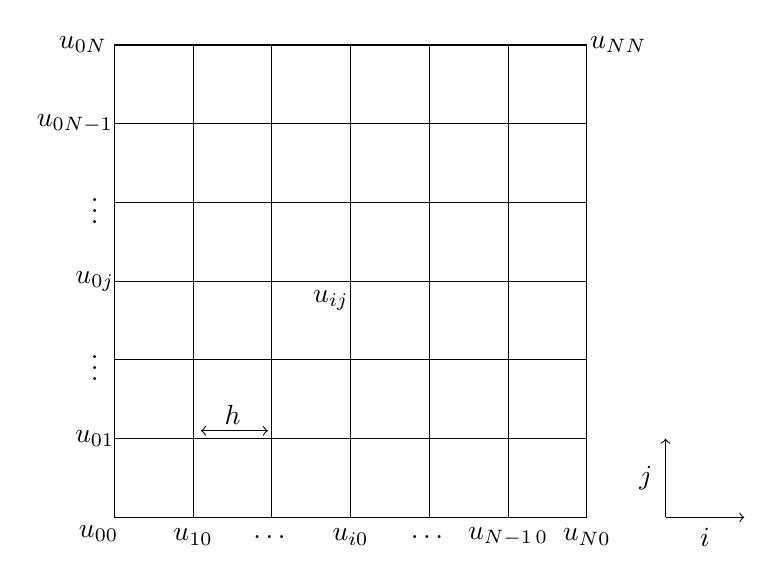
\begin{tikzpicture}
\draw (0,0) grid (6,6);
\node at (-0.2,-0.2) {$u_{00}$};
\node at (1,-0.25) {$u_{10}$};
\node at (2,-0.25) {$\dots$};
\node at (3,-0.25) {$u_{i0}$};
\node at (4,-0.25) {$\dots$};
\node at (5,-0.25) {$u_{N-1\,0}$};
\node at (6,-0.25) {$u_{N0}$};

\node at (-0.25,1) {$u_{01}$};
\node at (-0.25,2) {$\vdots$};
\node at (-0.25,3) {$u_{0j}$};
\node at (-0.25,4) {$\vdots$};
\node at (-0.5,5) {$u_{0N-1}$};
\node at (-0.4,6) {$u_{0N}$};

\node at (2.75,2.75) {$u_{ij}$};
\node at (6.4,6) {$u_{NN}$};

\draw[->] (7,0) -- (8,0);
\draw[->] (7,0) -- (7,1);
\node at (7.5,-0.25) {$i$};
\node at (6.75,0.5) {$j$};

\draw[<->] (1.1,1.1) -- (1.95,1.1);
\node at (1.5,1.3) {$h$};

\end{tikzpicture}
\centering
\caption{Discretised domain for $-u_{xx}-u_{yy}=f$.}
\end{figure}

The discretised form of this PDE can then be solved by computing the equation:
	\begin{equation}
	f_{ij} = -\frac{1}{h^2} \big( u_{i-1j} - 2u_{ij} + u_{i+1j} \big) - \frac{1}{h^2} \big( u_{ij-1} - 2u_{ij} + u_{ij+1} \big)
	\end{equation}
at each internal grid point, meaning the system has $n^2$ unknowns with $n=N-2$. 

The traditional approach to solving this discretised form would be to write (1.4) as:
	\begin{equation}
	f_{ij} = -\frac{1}{h^2} \big( u_{i-1j} + u_{ij-1} - 4u_{ij} + u_{i+1j} + u_{ij+1}  \big)
	\end{equation}
and then stack all unknowns $u_{ij}$ into a single vector $U$, resulting in the linear system $AU=F$. As stated previously, this ignores the underlying structure of the problem.

\subsection{Sylvester Equation}
A Sylvester equation is a matrix equation of the form $AX + XB = C$, where $A$ is a $n \times n$ matrix, $B$ is a $m \times m$ matrix, and $X$ and $C$ are $n \times m$ matrices. We can write (1.4) as a Sylvester equation in the form:
	\begin{equation}
	TU + UT = F
	\end{equation}
where $T$, $U$ and $F$ are of size $n \times n$.
Here $T=-\frac{1}{h^2} \, \text{tridiag}(1,-2,1)$ and $U_{ij} = u(x_i, y_j)$, where $(x_i, y_j)$ are interior grid nodes for $i,j=1,\dots,n$. The system has $n$ unknowns in each direction meaning there is a total of $n^2$ unknowns. The matrix equation is visualised below:
\begin{eqnarray}
\frac{-1}{h^2} 
\begin{pmatrix}
-2 & 1 & 0 & \dots & 0 & 0 \\
1 & -2 & 1 & \dots & 0 & 0 \\
0 & 1 & -2 & \dots & 0 & 0 \\
\vdots & \vdots & \vdots & \ddots & \vdots & \vdots \\
0 & 0 & 0 & \dots & -2 & 1 \\
0 & 0 & 0 & \dots & 1 & -2 \\
\end{pmatrix}
\begin{pmatrix}
u_{11} & u_{12} & \dots & u_{1j} & \dots & u_{1n} \\
u_{21} & u_{22} & \dots & u_{2j} & \dots & u_{2n} \\
\vdots & \vdots & \ddots & \vdots & \dots & \vdots \\
u_{i1} & u_{i2} & \dots & u_{ij} & \dots & u_{in} \\
\vdots & \vdots & \vdots & \vdots & \ddots & \vdots \\
u_{n1} & u_{n2} & \dots & u_{nj} & \dots & u_{nn}
\end{pmatrix} \nonumber \\ \nonumber
+
\begin{pmatrix}
u_{11} & u_{12} & \dots & u_{1j} & \dots & u_{1n} \\
u_{21} & u_{22} & \dots & u_{2j} & \dots & u_{2n} \\
\vdots & \vdots & \ddots & \vdots & \dots & \vdots \\
u_{i1} & u_{i2} & \dots & u_{ij} & \dots & u_{in} \\
\vdots & \vdots & \vdots & \vdots & \ddots & \vdots \\
u_{n1} & u_{n2} & \dots & u_{nj} & \dots & u_{nn}
\end{pmatrix}
\frac{-1}{h^2} 
\begin{pmatrix}
-2 & 1 & 0 & \dots & 0 & 0 \\
1 & -2 & 1 & \dots & 0 & 0 \\
0 & 1 & -2 & \dots & 0 & 0 \\
\vdots & \vdots & \vdots & \ddots & \vdots & \vdots \\
0 & 0 & 0 & \dots & -2 & 1 \\
0 & 0 & 0 & \dots & 1 & -2 \\
\end{pmatrix}
= F
\end{eqnarray}
There are a variety of methods that can be used to solve Sylvester equations. This project will explore and compare different methods for solving equations in this form. 

\newpage

\section{Scope and Schedule}
\subsection{Aim}
The aim of this project is to first study, implement and compare a range of matrix equation solvers. Following this, a specific problem will be derived with the help of my supervisor so that these solvers may be used and compared for a suitable application.

\subsection{Objectives}
The objectives of this project are as follows:
\begin{itemize}
\item To carry out an extensive, in-depth literature review on methods (both direct and iterative) for solving matrix equations from a wide range of sources. To decide which of these methods are appropriate to implement and to gain a solid understanding of how they work. 
\item To use and expand upon my programming experience to implement the chosen methods for solving matrix equations to solve the specified problem. 
\item To evaluate the implementation by comparing and contrasting the methods implemented to try to decide which is the best method for solving the given problem.
\item To derive a suitable application equation so that the methods studied in this project can be applied to a specific problem. 
\item To clearly present the work carried out during the project by using and building upon my report writing skills.
\end{itemize}

\subsection{Deliverables}
The deliverables of this project include:
\begin{itemize}
\item The final report that will include the details of the matrix solvers that have been studied, how the solvers were implemented, an evaluation and comparison of the implemented solvers, an analysis of how these solvers were used to solve the chosen application problem, and finally an evaluation of the success of the project.  
\item Code that successfully implements the chosen matrix solvers so that they solve the given problem.
\end{itemize}

\subsection{Methodology}
The methodology of this project will first involve studying academic publishings to gain an understanding of various methods for solving matrix equations. Python will be used as the programming language of choice for the implementation because of my familiarity with it, the extensive amount of documentation available for it and the excellent libraries it has available (e.g. NumPy and SciPy). GitHub will be used for version control and the final report will be written using \LaTeX. 

\subsection{Tasks, Milestones and Timeline}
The steps of this project will be divided into iterations, with the problem in each iteration becoming successively more complex and difficult to solve. This is because understanding is a key part of this project, and so each iteration will build on the understanding of the last. Each iteration will consist of studying and applying matrix methods to the problem, implementing them in Python to solve the problem, evaluating the results and write up. Also rough deadlines will be given for when each iteration should be completed by, to ensure the project is on track at any given stage.

The iterations are as follows:
\begin{itemize}
\item Introductory problem: $-u_{xx} - u_{yy} = 2 \pi^2 \sin{(\pi x)} \sin{(\pi y)}$ - deadline June 1st
\item Problem introducing uncertainty: $-\varepsilon u_{xx} - \varepsilon u_{yy} = 2 \pi^2 \sin{(\pi x)} \sin{(\pi y)}$ - deadline June 22nd
\item A Poisson equation on a surface defined by a height map (not yet derived) - deadline July 13th
\item Application reaction-diffusion equation (not yet derived) - deadline August 3rd
\end{itemize}

If the project deadlines are met the remaining time will be dedicated to project evaluation, write up and any possible project extensions.

\newpage

\section{Matrix Solvers}
For spatial domain $\mathcal{D} = \{(x,y) : 0 \leq x \leq 1, \; 0 \leq y \leq 1 \}$ and $u: \mathcal{D} \rightarrow \mathbb{R}$, let $u(x,y) = \sin{(\pi x)} \sin{(\pi y)}$ be the exact solution of the equation:
\begin{eqnarray}
-u_{xx} -u_{yy} = f & \text{ on } & \mathcal{D} \nonumber \\
u = 0 & \text{ on } & \partial \mathcal{D}
\end{eqnarray}

This gives:
\begin{eqnarray} 
u_{xx} = u_{yy} = - \pi^2 \sin{(\pi x)} \sin{(\pi y)} \nonumber \\
\implies f = 2 \pi^2 \sin{(\pi x)} \sin {(\pi y)}
\end{eqnarray}

The equation to be be solved is therefore:
\begin{eqnarray}
-u_{xx} -u_{yy} = 2 \pi^2 \sin{(\pi x)} \sin {(\pi y)} & \text{ on } & \mathcal{D} \nonumber \\
u = 0 & \text{ on } & \partial \mathcal{D}
\end{eqnarray}

Using the centred finite difference approximations ((1.2) and (1.3)) with uniform grid spacing $h$ to discretise the domain of this system, we have:
	\begin{eqnarray}
	& -\frac{1}{h^2} \big( u_{i-1j} - 2u_{ij} + u_{i+1j} \big) - \frac{1}{h^2} \big( u_{ij-1} - 2u_{ij} + u_{ij+1} \big) \nonumber \\ & = 2\pi^2 \sin(\pi x_i) \sin(\pi y_j)
	\end{eqnarray}
to be solved at each grid point for $i, j = 1, \dots n$, where $n$ is the total number of unknowns in each direction. The matrix form of this equation is therefore:
\begin{equation}
	TU + UT = F
	\end{equation}
where $T=-\frac{1}{h^2} \, \text{tridiag}(1,-2,1)$, $U_{ij} = u(x_i, y_j)$ and $F_{ij} = 2 \pi^2 \sin(\pi x_i) \sin(\pi y_j)$ are all matrices of size $n \times n$ and $(x_i, y_j)$ are interior grid nodes for $i,j=1,\dots,n$.

This form allows us to explore different methods for solving this equation and compare them to the exact solution $u = \sin(\pi x) \sin(\pi y)$. A plot of the exact solution, with $n=1000$, is given in Figure 3. 

\begin{figure}[H]
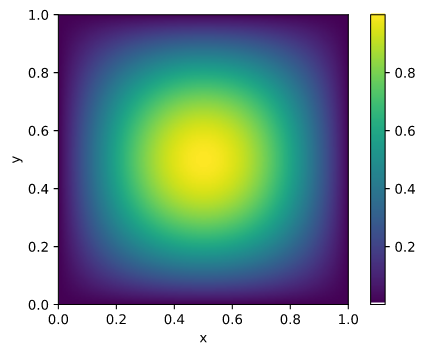
\includegraphics[scale=.5]{img/solution2.png}
\centering
\caption{Plot of the solution with $n=1000$.}
\end{figure} 

Throughout the following section, the following measurements are given to evaluate the performance of each of the methods implemented:
\begin{itemize}
\item $n$: The total number of unknowns in each direction for the system. The total number of unknowns is $n^2$.
\item Time(s): The time taken in seconds for the method to compute the solution to the problem.
\item $|| u - u_h ||_{L^\infty} $: Measures the maximum difference between the actual solution and computed solution for each $u$. Defined as:
 \[ || u - u_h ||_{L^\infty} = \text{max}_{ij} | u(x_i, y_i) - u_{ij} | \]
\item $|| u - u_h ||_{L^2} $: A measure of error that takes into account the difference between all actual and computed solutions, as well as the step size. Defined as:
\[ || u - u_h ||_{L^2} = \sqrt{h^2 \sum | u(x_i,y_j) - u_{ij} |^2} \]
\item Experimental order of convergence (eoc): Measures the rate of convergence of a method as the problem size is increased, which should approach 2 as the step size is increased. Defined as:
\[ \text{eoc}(i) = \frac{\log(\nicefrac{E_i}{E_{i-1}})}{\log(\nicefrac{h_i}{h_{i-1}})} \]
where $E_i$ is the error and $h_i$ is the mesh size at level $i$. 
\item Empirical order of growth (eog): Measures the order of growth of the execution time of an algorithm as the problem size is increased. Defined as:
\[ \text{eog}(i) = \frac{\log(\nicefrac{t_{i}}{t_{i-1}})}{\log(\nicefrac{n_{i}}{n_{i-1}})} \]
where $t_i$ is the total execution time and $n_i$ is the problem size at level $i$.
\end{itemize}

It is worth noting that as the total number of unknowns and hence the problem size is $n^2$, the best time complexity that an optimal solver can achieve is $O(n^2)$, as it must compute a solution for each unknown. 

\subsection{Direct Methods}

\subsubsection{Kronecker Product}
A naive approach to solving this system is to use the Kronecker product to rewrite (3.5) as a standard vector linear system. The Sylvester equation $AX + XB = C$ can be written as the standard vector linear system:
\begin{equation}
\mathcal{A}x = c
\end{equation}
with $\mathcal{A} = I \otimes A + B^* \otimes I$, where $I$ is the identity matrix, $B^*$ denotes the conjugate transpose of $B$, $x = \text{vec}(X)$ and $c = \text{vec}(C)$.\footnote{The vec operator reshapes a matrix into a vector by stacking the columns one after another.}

For the system in (3.6), we have $A=B=T$, $X=U$, $C=F$ and $T=T^*$, so the standard linear system is:
\begin{equation}
\mathcal{T}u = \mathcal{F}
\end{equation}
where $\mathcal{F} = \text{vec}(F)$, $\mathcal{T} = I \otimes T + T \otimes I$ and $u = \text{vec}(U)$. 

This is the exact linear system that would be obtained from equation (1.5), i.e. stacking all unknowns $u_{ij}$ into a single vector in the first place. Since the matrix $\mathcal{T}$ is sparse, this equation can be solved using a standard direct sparse solver. This approach provides a good base case for comparison. Results solving this linear system using the direct sparse solver \texttt{sparse.linalg.spsolve} from the SciPy library are shown in Table 1. As can be seen from the results, both errors decrease as the problem size $n$ is increased. The eoc is very close to 2 for all $n$, demonstrating the convergence of the algorithm. As $n$ is increased the eog grows beyond $3$, which shows this algorithm has worse than cubic time complexity for large $n$. 

\begin{table}[H]
\centering
\begin{tabular}{|c|c|c|c|c|c|}
\hline
$n$ & Time(s) & $|| u - u_h ||_{L^{\infty}}$ &$|| u - u_h ||_{L^{2}}$ & eoc & eog \\
\hline
125 & 0.18141 & $5.1807 \times 10^{-5}$ & $2.5904 \times 10^{-5}$ & - & - \\
250 & 0.60371 & $1.3054 \times 10^{-5}$ & $6.5275 \times 10^{-6}$ & 2.0001 & 1.7346 \\
500 & 4.1663 & $3.2767 \times 10^{-6}$ & $1.6384 \times 10^{-6}$ & 1.9999 & 2.7868 \\
1000 & 36.113 & $8.2082 \times 10^{-7}$ & $4.1041 \times 10^{-7}$ & 2.0000 & 3.1157 \\
2000 & 404.48 & $2.0539 \times 10^{-7}$ & $1.0267 \times 10^{-7}$ & 2.0001 & 3.4855 \\
\hline
\end{tabular}
\captionsetup{justification=centering}
\caption{Results obtained from solving the linear system $\mathcal{A} x = c$ using the direct solver  \texttt{sparse.linalg.spsolve} from the SciPy library.}
\end{table}

\subsubsection{Bartels-Stewart Algorithm}
The Bartels-Stewart algorithm \cite{Bartels} can be used to solve the Sylvester equation $AX + XB = C$. In the general case the algorithm is as follows:
\begin{enumerate}
\item Compute the Schur forms $A^* = PRP^*$ and $B=QSQ^*$
\item Solve $R^*V + VS = P^*CQ$ for $V$
\item Compute $X=PVQ^*$
\end{enumerate}
where $A^*$ denotes the conjugate transpose of $A$.

In this case $A=B=T$, $T=T^*$, $X=U$ and $C=F$ so the algorithm is as follows:
\begin{enumerate}
\item Compute the Schur form $T=PRP^*$
\item Solve $R^*V + VR = P^*FP$ for $V$
\item Compute $U=PVP^*$
\end{enumerate}

Results using this algorithm are shown in Table 2. These results show that both errors decrease as $n$ is increased. Also the eoc is close enough to 2 to conclude that this algorithm converges. The eog demonstrates that this algorithm has an approximate cubic time complexity. 

\begin{table}[H]
\centering
\begin{tabular}{|c|c|c|c|c|c|}
\hline
$n$ & Time(s) & $|| u - u_h ||_{L^{\infty}}$ &$|| u - u_h ||_{L^{2}}$ & eoc & eog \\
\hline
125 & 1.2486 & $5.1807 \times 10^{-5}$ & $2.5904 \times 10^{-5}$ & - & - \\
250 & 9.6712 & $1.3054 \times 10^{-5}$ & $6.5275 \times 10^{-6}$ & 2.0001 & 2.9124 \\
500 & 77.888 & $3.2767 \times 10^{-6}$ & $1.6384 \times 10^{-6}$ & 1.9999 & 3.0096 \\ 
1000 & 640.22 & $8.2088 \times 10^{-7}$ & $4.1044 \times 10^{-7}$ & 2.0000 & 3.0391 \\
2000 & 5093.1 & $2.0467 \times 10^{-7}$ & $1.0237 \times 10^{-7}$ & 2.0052 & 2.9919 \\
\hline
\end{tabular}
\caption{Results using the Bartels-Stewart algorithm.}
\end{table}

By breaking this algorithm down into its component parts, we can time each step to see which is the most costly. The results of doing so are given in Table 3, where the steps are:

\begin{enumerate}
\item Compute the Schur form $T=PRP^*$ (using \texttt{linalg.schur} from the SciPy library)
\item Solve the $R^*V + VR = P^*FP$ for $V$, which is a triangular system
\item Compute the solution $U=PVP^*$
\end{enumerate}

As can be seen from the results in Table 3, the most costly part of the algorithm is by far the second step, which is due to the fact that solving the triangular system uses back substitution which requires multiple nested \texttt{for} loops.

\begin{table}[H]
\centering
\begin{tabular}{|c|c|c|c|c|}
\hline
$n$ & 1 & 2 & 3 & Total \\
\hline
125 & 0.012667 & 1.2357 & 0.00023031 & 1.2486 \\
250 & 0.048434 & 9.6218 & 0.0010102 & 9.6712 \\
500 & 0.26262 & 77.619 & 0.0064600 & 77.888 \\ 
1000 & 0.083478 & 639.34 & 0.043818 & 640.22 \\
2000 & 5.1290 & 5087.5 & 0.41275 & 5093.1 \\
\hline
\end{tabular}
\caption{Timings for each step using the Bartels-Stewart algorithm.}
\end{table}

The SciPy library has a built in solver for solving Sylvester equations, \texttt{linalg.solve \_sylvester}, which uses the Bartels-Stewart algorithm. Results using this solver are given in Table 4. The errors here are similar to the errors given in Table 2. Again the eoc is close enough to 2 to conclude that this algorithm converges. However, the eog seems to vary depending on the problem size $n$. 

\begin{table}[H]
\centering
\begin{tabular}{|c|c|c|c|c|c|}
\hline
$n$ & Time(s) & $|| u - u_h ||_{L^{\infty}}$ &$|| u - u_h ||_{L^{2}}$ & eoc & eog \\
\hline
125 & 0.059959 & $5.1807 \times 10^{-5}$ & $2.5904 \times 10^{-5}$ & - & - \\
250 & 0.11421 & $1.3054 \times 10^{-5}$ & $6.5275 \times 10^{-6}$ & 2.0001 & 0.92964 \\
500 & 1.9383 & $3.2767 \times 10^{-6}$ & $1.6384 \times 10^{-6}$ & 1.9999 & 4.0850  \\
1000 & 4.0920 & $8.2084 \times 10^{-7}$ & $4.1042 \times 10^{-7}$ & 2.0000 & 1.0780 \\
2000 & 32.029 & $2.0503 \times 10^{-7}$ & $1.0259 \times 10^{-7}$ & 2.0027 & 2.9685  \\
4000 & 279.95 & $4.9949 \times 10^{-8}$ & $2.4876 \times 10^{-8}$ & 2.0377 & 3.1277  \\
\hline
\end{tabular}
\caption{Results using SciPy's \texttt{linalg.solve\_sylvester}.}
\end{table}

As can be seen from the results above, using the built-in SciPy solver results in a significant speed-up in time as $n$ is increased. This is likely because it makes use of of LAPACK, which is an optimised software library for solving linear algebra problems.


\subsubsection{Similarity Transformation}
A similarity transformation \cite{Simoncini} can be used to solve the Sylvester equation $AX + XB = C$. Assuming matrices $A$ and $B$ can be diagonalised, let $P^{-1}AP = \text{diag}(\lambda_1, \dots, \lambda_n)$ and $Q^{-1}BQ = \text{diag}(\mu_1, \dots, \mu_m)$, where $\lambda_1, \dots, \lambda_n$ are the eigenvalues of $A$, $\mu_1, \dots, \mu_m$ are the eigenvalues values of $B$ and the columns of $P$ and $Q$ are the eigenvectors of $A$ and $B$, respectively. Letting $\tilde{C} = P^{-1}CQ$, the solution is then:
\[ X = P \tilde{X} Q^{-1}, \text{ with } \tilde{x}_{ij} = \frac{\tilde{c}_{ij}}{\lambda_i + \mu_j} \]

In this case, $A=B=T$, $X=U$ and $C=F$ so $P=Q$ and $P^{-1}TP = \text{diag}(\lambda_1, \dots, \lambda_n)$, where $\lambda_1, \dots, \lambda_n$ are the eigenvalues of $T$ and the columns of $P$ are the eigenvectors of $T$. Letting $\tilde{F}=P^{-1}FP$, the solution is then:
\[ U = P \tilde{U} P^{-1}, \text{ with } \tilde{u}_{ij} = \frac{\tilde{f}_{ij}}{\lambda_i + \lambda_j} \]

\subsubsection*{Using numpy.linalg.eig}
Using the method above, the eigenvalues and eigenvectors can be computed using NumPy's \texttt{linalg.eig} function. The results doing this are given in Table 5. The errors are again similar to the previous methods. However, here the eoc moves away from 2 as $n$ is increased. This is likely due to the fact that there is no general formula for calculating eigenvalues and eigenvectors for an arbitrary matrix, meaning the eigenvalues and eigenvectors are most likely approximated by NumPy's \texttt{linalg.eig}. It is likely that the approximations become less accurate as $n$ is increased. The eog here is however slightly better than the previous methods. 

\begin{table}[H]
\centering
\begin{tabular}{|c|c|c|c|c|c|}
\hline
$n$ & Time(s) & $|| u - u_h ||_{L^{\infty}}$ &$|| u - u_h ||_{L^{2}}$ & eoc & eog \\
\hline
125 & 0.034534 & $5.1802 \times 10^{-5}$ & $2.5904 \times 10^{-5}$ & -  & - \\
250 & 0.13690 & $1.3054 \times 10^{-5}$ & $6.5275 \times 10^{-6}$ & 2.0000 & 1.9870  \\
500 & 0.59718 & $3.2767 \times 10^{-6}$ & $1.6384 \times 10^{-6}$ & 1.9999 & 2.1250  \\
1000 & 2.2211 & $8.2086 \times 10^{-7}$ & $4.1043 \times 10^{-7}$ & 1.9999 & 1.8950  \\
2000 & 11.571 & $2.0467 \times 10^{-7}$ & $1.0237 \times 10^{-7}$ & 2.0053 & 2.3812  \\
4000 & 70.984 & $4.9966 \times 10^{-8}$ & $2.4876 \times 10^{-8}$ & 2.0350 & 2.6170  \\
8000 & 466.83 & $8.6360 \times 10^{-9}$ & $4.1223 \times 10^{-9}$ & 2.5330 & 2.7173  \\
\hline
\end{tabular}
\captionsetup{justification=centering}
\caption{Results using a similarity transformation, calculating the eigenvalues and eigenvectors using \texttt{numpy.linalg.eig}.}
\end{table}

Similarly to the Bartels-Stewart algorithm, this method can be split into component parts and each part can be timed, to see which part is the most costly. The steps of the method are:
\begin{enumerate}
\item Calculate eigenvalues and eigenvectors of $T$
\item Diagonalise $T$ (i.e. calculate $P$ and $P^{-1}$)
\item Calculate $\tilde{F}=P^{-1}FP$
\item Calculate $\tilde{U}$, where $\tilde{u}_{ij} = \frac{\tilde{f}_{ij}}{\lambda_i + \lambda_j}$
\item Calculate solution $U=P \tilde{U}P^{-1}$
\end{enumerate}

The results of doing so are shown in Table 6.

\begin{table}[H]
\centering
\begin{tabular}{|c|c|c|c|c|c|c|}
\hline
$n$ & 1 & 2 & 3 & 4 & 5 & Total \\
\hline
125 & 0.013860 & 0.00042105 & 0.00075817 & 0.018881 & 0.00061440 & 0.034534 \\
250 & 0.052402 & 0.00068998 & 0.0026329 & 0.078654 & 0.0025253 & 0.13690 \\
500 & 0.25900 & 0.0020170 & 0.013870 & 0.30815 & 0.014147 & 0.59718 \\
1000 & 0.91819 & 0.0011129 & 0.084650 & 1.1328 & 0.084323 & 2.2211 \\
2000 & 5.8236 & 0.0035102 & 0.61534 & 4.5150 & 0.61360 & 11.571 \\
4000 & 43.651 & 0.0074658 & 4.6290 & 18.071 & 4.6257 & 70.984 \\
8000 & 325.30 & 0.027416 & 35.464 & 70.695 & 35.345 & 466.83 \\
\hline
\end{tabular}
\captionsetup{justification=centering}
\caption{Timing results for each step of the similarity transformation method, calculating the eigenvalues and eigenvectors using \texttt{numpy.linalg.eig}.}
\end{table}

\subsubsection*{Calculating eigenvalues and eigenvectors explicitly}

As can be seen from the results in Table 6, the most costly part of this method is calculating the eigenvalues and eigenvectors. As $T$ is a matrix in Toeplitz form, the eigenvalues and eigenvectors can be calculated directly as:
\[ \lambda_i = \frac{2}{h^2} \Big( \cos \Big( \frac{i \pi}{n+1} \Big) - 1 \Big) \]
and:
\[ t_{ij} = \sqrt{\frac{2}{n+1}} \sin \Big( \frac{ij \pi}{n+1}  \Big) \]

Results using this method for calculating the eigenvalues are eigenvectors are given in Table 7, and timings for each step are given in Table 8. Similar errors are given by this method, however now the eoc is much closer to 2 as $n$ is increased. The eog is also significantly less demonstrating that using this algorithm and computing the eigenvalues explicity achieves a near square time complexity. 

\begin{table}[H]
\centering
\begin{tabular}{|c|c|c|c|c|c|}
\hline
$n$ & Time(s) & $|| u - u_h ||_{L^{\infty}}$ &$|| u - u_h ||_{L^{2}}$ & eoc & eog\\
\hline
125 & 0.080673 & $5.1807 \times 10^{-5}$ & $2.5904 \times 10^{-5}$ & - & -  \\
250 & 0.30396 & $1.3054 \times 10^{-5}$ & $6.5275 \times 10^{-6}$ & 2.0001 & 1.9137  \\
500 & 1.2021 & $3.2767 \times 10^{-6}$ & $1.6384 \times 10^{-6}$ & 1.9999 & 1.9836 \\
1000 & 5.5904 & $8.2082 \times 10^{-7}$ & $4.1041 \times 10^{-7}$ & 2.0000 & 2.2174  \\
2000 & 20.247 & $2.0541 \times 10^{-7}$ & $1.0270 \times 10^{-7}$ & 2.0000 & 1.8567 \\
4000 & 82.243 & $5.1314 \times 10^{-8}$ & $2.5656 \times 10^{-8}$ & 2.0018 & 2.0222  \\
8000 & 360.35 & $1.2814 \times 10^{-8}$ & $6.4065 \times 10^{-9}$ & 2.0020 & 2.1314  \\
\hline
\end{tabular}
\captionsetup{justification=centering}
\caption{Results using a similarity transformation, calculating the eigenvalues and eigenvectors explicity.}
\end{table}

\begin{table}[H]
\centering
\begin{tabular}{|c|c|c|c|c|c|c|}
\hline
$n$ & 1 & 2 & 3 & 4 & 5 & Total \\
\hline
125 & 0.057252 & 0.00025916 & 0.0045545 & 0.018010 & 0.00059748 & 0.080673 \\
250 & 0.21954 & 0.00047016 & 0.0081279 & 0.073295 & 0.0025220 & 0.30396 \\ 
500 & 0.88125 & 0.0012608 & 0.018555 & 0.28724 & 0.013819 & 1.2021  \\
1000 & 3.7073 & 0.00096869 & 0.67056 & 1.1304 & 0.081200 & 5.5904 \\
2000 & 13.812 & 0.0092294 & 1.3690 & 4.4495 & 0.60793 & 20.247 \\
4000 & 54.907 & 0.0068946 & 4.9050 & 17.381 & 4.5936 & 82.243 \\
8000 & 217.26 & 0.026015 & 35.357 & 71.581 & 36.129 & 360.35 \\
\hline
\end{tabular}
\captionsetup{justification=centering}
\caption{Timing results for each step of the similarity transformation method, calculating the eigenvalues and eigenvectors explicitly.}
\end{table}

As can be seen from the results in Table 8, calculating the eigenvalues and eigenvectors explicitly  outperforms calculating them using the NumPy library when $n$ is large.

\subsubsection{Shifted System}
A projection method \cite{Simoncini} can be used on a Sylvester equation $AX + XB =C$ by decomposing $B$ to obtain $n$ linear systems, each of which can be solved simultaneously (and in parallel) to obtain the solution $X$. The steps of this method are as follows:
\begin{enumerate}
\item Compute $B = WSW^{-1}$, where $S = \text{diag}(s_1, \dots, s_n)$ are the eigenvalues of $B$ and the columns of $W$ are the eigenvectors of $B$
\item Compute $\hat{C} = CW$
\item For $i=1$ to $n$, solve the system $(A+s_i I)(\hat{X})_i = (\hat{C})_i$
\item Compute solution $X = \hat{X}W$
\end{enumerate}
where $(\hat{X})_i$ denotes the $i^{\text{th}}$ column of $\hat{X}$.

In the case of $TU + UT = F$, the steps are as follows:
\begin{enumerate}
\item Compute $T = WSW^{-1}$, where $S = \text{diag}(s_1, \dots, s_n)$ are the eigenvalues of $T$ and the columns of $W$ are the eigenvectors of $T$
\item Compute $\hat{F} = FW$
\item For $i=1$ to $n$, solve the system $(T+s_i I)(\hat{U})_i = (\hat{F})_i$
\item Compute solution $U = \hat{U}W$
\end{enumerate}

Results using this method are given in Table 9. The errors are approximately the same as the errors given previously. The eoc is approximately 2 and the eog is $> 3$ for large $n$ demonstrating that this algorithm converges with a worse than cubic time complexity. 
\begin{table}[H]
\centering
\begin{tabular}{|c|c|c|c|c|c|}
\hline
$n$ & Time(s) & $|| u - u_h ||_{L^{\infty}}$ &$|| u - u_h ||_{L^{2}}$ & eoc & eog \\
\hline
125 & 0.092085 & $5.1807 \times 10^{-5}$ & $2.5904 \times 10^{-5}$ & - & - \\
250 & 0.43609 & $1.3054 \times 10^{-5}$ & $6.5274 \times 10^{-6}$ & 2.0001 & 2.2436 \\
500 & 2.1851 & $3.2767 \times 10^{-6}$ & $1.6384 \times 10^{-6}$ & 1.9999 & 2.3250 \\
1000 & 19.498 & $8.2082 \times 10^{-7}$ & $4.1041 \times 10^{-7}$ & 2.0000 & 3.1576 \\
2000 & 194.13 & $2.0541 \times 10^{-7}$ & $1.0271 \times 10^{-7}$ & 2.0000 & 3.3156 \\
4000 & 2452.5 & $5.1347 \times 10^{-8}$ & $2.5674 \times 10^{-8}$ & 2.0009 & 3.6592  \\
\hline
\end{tabular}
\captionsetup{justification=centering}
\caption{Results using a projection method to solve $n$ linear systems.}
\end{table}

The steps of this method can also be broken down into component parts and each part timed. The results of doing so are given in Table 10. Unsuprisingly, the most costly part of the algorithm is solving the $n$ linear systems. 

\begin{table}[H]
\centering
\begin{tabular}{|c|c|c|c|c|c|}
\hline
$n$ & 1 & 2 & 3 & 4 & Total \\
\hline
125 & 0.057421 & 0.0043032 & 0.3028 & $7.1764 \times 10^{-7}$ & 0.092085 \\
250 & 0.23967 & 0.0041912 & 0.19177 & 0.00046206 & 0.43609  \\
500 & 0.85408 & 0.0079994 & 1.3200 & 0.0030336 & 2.1851 \\
1000 & 3.3709 & 0.026276 & 16.079 & 0.021675 & 19.498 \\
2000 & 13.278 & 0.50065 & 180.81 & 0.16621 & 194.13 \\
4000 & 53.300 & 1.8301 & 2396.1 & 1.2866 & 2452.5  \\
\hline
\end{tabular}
\captionsetup{justification=centering}
\caption{Timing results of each step using a projection method to solve $n$ linear systems.}
\end{table}

\subsection{Iterative Methods}

\subsubsection{Kronecker Product}
Similarly to Section 3.1.1, the Kronecker product can be used to write the matrix equation as a standard vector linear system. A a standard iterative solver can then be used to solve the system, which can provide a base case for comparison. Results using \texttt{scipy.sparse.linalg.cg}, which is a sparse solver that uses the conjugate gradient iterative method, are given in Table 11, using a convergence tolerance of $10^{-9}$. The results show errors similar to all the direct methods. The eoc demonstrates that the algorithm converges very well. Although this algorithm is much faster than all the previous direct methods, the eog demonstrates that when $n$ is significantly large, the algorithm exhibits a worse than cubic time complexity, which is shown here when $n=8000$.  

\begin{table}[H]
\centering
\begin{tabular}{|c|c|c|c|c|c|}
\hline
$n$ & Time(s) & $|| u - u_h ||_{L^{\infty}}$ &$|| u - u_h ||_{L^{2}}$ & eoc & eog \\
\hline
125 & 0.014182 & $5.1807 \times 10^{-5}$ & $2.5904 \times 10^{-5}$ & - & - \\
250 & 0.042605 & $1.3054 \times 10^{-5}$ & $6.5275 \times 10^{-6}$ & 2.0001 & 1.5870 \\
500 & 0.14136 & $3.2767 \times 10^{-6}$ & $1.6384 \times 10^{-6}$ & 1.9999 & 1.7303 \\
1000 & 0.54308 & $8.2082 \times 10^{-7}$ & $4.1041 \times 10^{-7}$ & 2.0000 & 1.9418 \\
2000 & 2.3162 & $2.0541 \times 10^{-7}$ & $1.0271 \times 10^{-7}$ & 2.0000 & 2.0925 \\
4000 & 9.8487 & $5.1379 \times 10^{-8}$ & $2.5689 \times 10^{-8}$ & 2.0000 & 2.0882 \\
8000 & 103.34 & $1.2848 \times 10^{-8}$ & $6.4239 \times 10^{-9}$ & 2.0000 & 3.3913 \\
\hline
\end{tabular}
\captionsetup{justification=centering}
\caption{Results obtained from solving the linear system $\mathcal{A} x = c$ using the iterative solver  \texttt{sparse.linalg.cg} from the SciPy library.}
\end{table}

\subsubsection{Gradient Based Method}
In \cite{Zhou} a gradient based method for solving Sylvester equations is given. The equation $TU + UT = F$ can be written as two recursive sequences:
	\begin{equation}
	U_k^{(1)} = U_{k-1}^{(1)} + \kappa T(F-TU_{k-1}^{(1)} - U_{k-1}^{(1)}T)
	\end{equation}
	\begin{equation}
	U_k^{(2)} = U_{k-1}^{(2)} + \kappa (F-TU_{k-1}^{(2)} - U_{k-1}^{(2)}T)T
	\end{equation}
where $\kappa$ represents the relative step size. The approximate solution $U_k$ is taken as the average of these two sequences:
	\begin{equation}
	U_k = \frac{U_k^{(1)} + U_k^{(2)}}{2}
	\end{equation}
This solution only converges if:
	\begin{equation}
	0 < \kappa < \frac{1}{\lambda_{\text{max}}(T^2)} 
	\end{equation}
where $\lambda_{\text{max}}(T^2)$ denotes the maximum eigenvalue of $T^2$. Using the method given previously for calculating eigenvalues we can compute:
\begin{equation}
\lambda_{\text{max}}(T^2) = \frac{4}{h^4} \text{max} \Big( \big( \cos{\Big(\frac{i \pi}{n+1} \Big) } -1 \big)^2 \Big)
\end{equation}
$\lambda_{\text{max}}(T^2)$ therefore scales with $\frac{1}{h^4}$ meaning its reciprocal scales with $h^4$, implying $\kappa$ will need to be significantly small as $n$ is increased for the solution to converge. Even for small values of $n$, this is impractical and therefore this method is not appropriate for solving this equation.

\subsubsection{Modified Conjugate Gradient}
In \cite{Hou} a modified conjugate gradient (MCG) algorithm is proposed, which is adapted for solving Sylvester Equations. The algorithm is as follows:
\begin{enumerate}
\item Choose initial guess $X^{(0)}$, let $k=0$ and calculate:
	\begin{itemize}
	\item $R^{(0)} = F - AX^{(0)} - X^{(0)}B$
	\item $Q^{(0)} = A^T R^{(0)} + R^{(0)} + R^{(0)} B^T$
	\item $Z^{(0)} = Q^{(0)}$
	\end{itemize}
\item If $R^{(k)} = 0$, or $R^{(k)} \neq 0$ but $Z^{(k)} = 0$, stop. Else, calculate:
\[ \gamma_k = \frac{[R^{(k)}, R^{(k)}]}{[Z^{(k)}, Z^{(k)}]} \]
where $[R,R] = \text{tr}(R^T R)$ is the trace of the matrix $R^T R$.
\item Calculate:
	\begin{itemize}
	\item $R^{(k+1)} = F - AX^{(k+1)} - X^{(k+1)} B$
	\item $Q^{(k+1)} = A^T R^{(k+1)} + R^{(k+1)} + R^{(k+1)} B^T$
	\end{itemize}
	and return to Step 2.
\end{enumerate}
\newpage

\section{Uncertainty}
Uncertainty can arise in partial differential equations if, for example, coefficients, boundary conditions or initial conditions are unknown. A solution to dealing with uncertainty is to model unknown parameters as random variables, and then appropriate methods can be used to solve the system. 

\subsection{Single Parameter}
The simplest way to introduce uncertainty into a partial differential equation is by introducing a single unknown parameter. Define the spatial domain $\mathcal{D}$ as $\mathcal{D} = \{(x,y) : 0 \leq x \leq 1, \; 0 \leq y \leq 1 \}$, and let $\Omega$ denote the sample space. We can introduce an unknown coefficient $\varepsilon(\omega)$, where $\omega \in \Omega$ and $\varepsilon: \Omega \rightarrow \mathbb{R}$ is uniformly distributed over the interval $[-1,1]$ with $\varepsilon \neq 0$. Let $u(x,y,\varepsilon) = \sin(\pi x)\sin(\pi y) + \varepsilon \sin(3 \pi x) \sin(5 \pi y)$ be the exact solution of the equation:
\begin{eqnarray}
-\varepsilon u_{xx} -\varepsilon u_{yy} = f & \text{ on } & \mathcal{D} \nonumber \\
u = 0 & \text{ on } & \partial \mathcal{D}
\end{eqnarray}
which gives:
\begin{eqnarray}
u_{xx} = -\pi^2 \sin(\pi x) \sin(\pi y) - 9\pi^2 \varepsilon \sin(3\pi x) \sin(5\pi y) \nonumber \\
u_{xx} = -\pi^2 \sin(\pi x) \sin(\pi y) - 25\pi^2 \varepsilon \sin(3\pi x) \sin(5\pi y) \nonumber \\
\implies f = 2\pi^2 \sin(\pi x) \sin(\pi y) + 34\pi^2 \varepsilon \sin(3\pi x) \sin(5\pi y)
\end{eqnarray}

The equation to be solved is therefore:
\begin{eqnarray}
- \varepsilon u_{xx} - \varepsilon u_{yy} = 2\pi^2 \varepsilon \sin(\pi x) \sin(\pi y)+ 34 \pi^2 \varepsilon^2 \sin(3 \pi x) \sin(5 \pi y) & \text{ on } & \mathcal{D} \times \Omega \nonumber \\
u = 0 & \text{ on } & \partial \mathcal{D} \times \Omega \nonumber \\
\end{eqnarray}

By discretising the domain using the centred finite difference approximations, (4.3) can be formed as a matrix equation:
\begin{equation}
TU + UT = F
\end{equation}
with $T = -\frac{\varepsilon}{h^2} \text{tridiag}(1,-2,1)$, $U = u(x_i, y_j)$ and $F = 2\pi^2 \varepsilon \sin(\pi x_i) \sin(\pi y_j)+ 34 \pi^2 \varepsilon^2 \sin(3 \pi x_i) \sin(5 \pi y_j)$. This problem is significantly harder to solve accurately and efficiently than the problem in Section 3 due to the fact that $\varepsilon$ is an unknown, random coefficient.

As $\varepsilon$ is unknown, the exact solution to (4.3) cannot be computed and therefore solutions to (4.4) cannot be compared to the true solution. Instead, certain quantities of interest can be computed using the probability density function $\rho(\omega)$ of $\varepsilon$. Firstly, the expectation $\mathbb{E}[u]$ can be computed as:
\begin{equation}
\mathbb{E}[u] = \int u(x,y,\varepsilon) \rho(\omega) d \omega
\end{equation}

The variance $\text{Var}[u]$ can also be computed as:
\begin{equation}
\text{Var}[u] = \int \left(u(x,y,\varepsilon) - \mathbb{E}[u] \right)^2 \rho(\omega) d \omega
\end{equation}
and the standard deviation $\text{Std}[u]$ as:
\begin{equation}
\text{Std}[u] = \sqrt{\text{Var}[u]}
\end{equation}

As $\varepsilon$ is uniformly distributed over the interval $[-1,1]$, it has a probability distribution function:
\begin{equation}
\rho(\omega) = \frac{1}{2}
\end{equation}

The expectation is therefore:
\begin{equation}
\begin{split}
\mathbb{E}[u] = & \frac{1}{2} \int_{-1}^1 \sin(\pi x)\sin(\pi y) + \varepsilon \sin(3 \pi x) \sin(5 \pi y) d \omega \\
= & \frac{1}{2} \left[\varepsilon \sin(\pi x) \sin(\pi y) + \frac{\varepsilon^2}{2} \sin(3 \pi x) \sin(5 \pi y)\right]_{-1}^{1} \\
= & \sin(\pi x) \sin(\pi y)
\end{split}
\end{equation}

and the variance is:
\begin{equation}
\begin{split}
\text{Var}[u] = & \frac{1}{2} \int_{-1}^1 (\sin(\pi x) \sin(\pi y) + \varepsilon \sin(3 \pi x) \sin(5 \pi y) - \sin(\pi x) \sin(\pi y))^2 d \omega \\
= & \frac{1}{2} \int_{-1}^1 \varepsilon^2 \sin^2 (3 \pi x) \sin^2 (5 \pi y) d \omega \\
= & \frac{1}{2} \left[ \frac{\varepsilon^3}{3} \sin^2 (3 \pi x) \sin^2 (5 \pi y) \right]_{-1}^1 \\
= & \frac{1}{3} \sin^2 (3 \pi x) \sin^2 (5 \pi y)
\end{split}
\end{equation}

which gives the standard deviation as:
\begin{equation}
\text{Std}[u] = \frac{1}{\sqrt{3}} \sin(3 \pi x) \sin(5 \pi y)
\end{equation}

Once solutions to (4.4) are computed they can be compared to the known expectation, variance and standard deviation.

\subsubsection{Monte Carlo}
A simple way of solving (4.4) is to use the Monte Carlo method. The Monte Carlo method works by taking $M$ random samples of $\varepsilon$ over its range, and then solves (4.4) for each of these samples. 
This allows the most effective method from Section 3 to be used as a `black box' strategy. Once solved, the expectation can be calculated as:
\begin{equation}
\mathbb{E}_M[u] = \frac{1}{M} \sum_{i=1}^M u_h (x, y, \varepsilon)
\end{equation}
where $M$ is the number of samples used in the Monte Carlo method and $u_h$ is the solution obtained from the finite difference method using a mesh of size $h$. This expectation is denoted as $\mathbb{E}_M[u]$ to indicate that it is the expectation computed from the Monte Carlo method, rather than the known expectation (that is, (4.5)). 

Similarly, the variance and standard deviation can also be computed as:
\begin{equation}
\text{Var}_M[u] = \frac{1}{M-1}\sum_{i=1}^M (u_h - \mathbb{E}_M[u])^2
\end{equation}
and:
\begin{equation}
\text{Std}_M[u] = \sqrt{\text{Var}[u]}
\end{equation}


Any of these quantites can then be chosen and compared to the known values as a measure of error for the problem. By choosing the mean we can measure the error as:
\begin{equation}
\begin{split}
\text{Error} = & \bigg{|} \bigg{|} \mathbb{E}[u] - \mathbb{E}_M[u] \bigg{|} \bigg{|} \\
= & \bigg{|} \bigg{|} \mathbb{E}[u] - \frac{1}{M} \sum_{i=1}^M u_h (x, y, \varepsilon) \bigg{|}\bigg{|}
\end{split}
\end{equation}


\subsubsection{Stochastic Galerkin}

\subsection{Multiple Parameters}

\newpage

\bibliographystyle{abbrv}
\bibliography{matrixsolvers}

\end{document}